\chapter{Mining additional perspectives}

\section{Introduction}

Until now, process mining has focused primarily on events recorded in an event log. However, significant insights can also be derived from examining \textbf{who} performs specific tasks or activities. This introduces new perspectives into the process mining, such as the resource, data, and time perspectives.

\subsection{Preprocessing and Filtering}
Before analyzing the event logs, it is essential to pre-process and filter the data to ensure its quality. This includes:
\begin{itemize}
    \item Removing irrelevant or noisy events,
    \item Organizing the data for visualization and analysis.
\end{itemize}

\section{Visualizing Data: Dotted Charts and Helicopter View}

\subsection{Dotted Chart}
A \textbf{dotted chart} is a graphical representation of event logs:
\begin{itemize}
    \item The \textbf{x-axis} represents timestamps,
    \item The \textbf{y-axis} represents trace numbers.
\end{itemize}

This chart helps to visualize how individual customers or cases progress over time. For example:
\begin{itemize}
    \item Denser lines indicate frequent activities,
    \item Sparse dots indicate rare or exceptional events.
\end{itemize}


\subsection{Helicopter View}
By varying symbols, colors and shapes in the dotted chart, a \textbf{helicopter view} can be created, providing insight into trends and variations in activities over time.
\begin{center}
    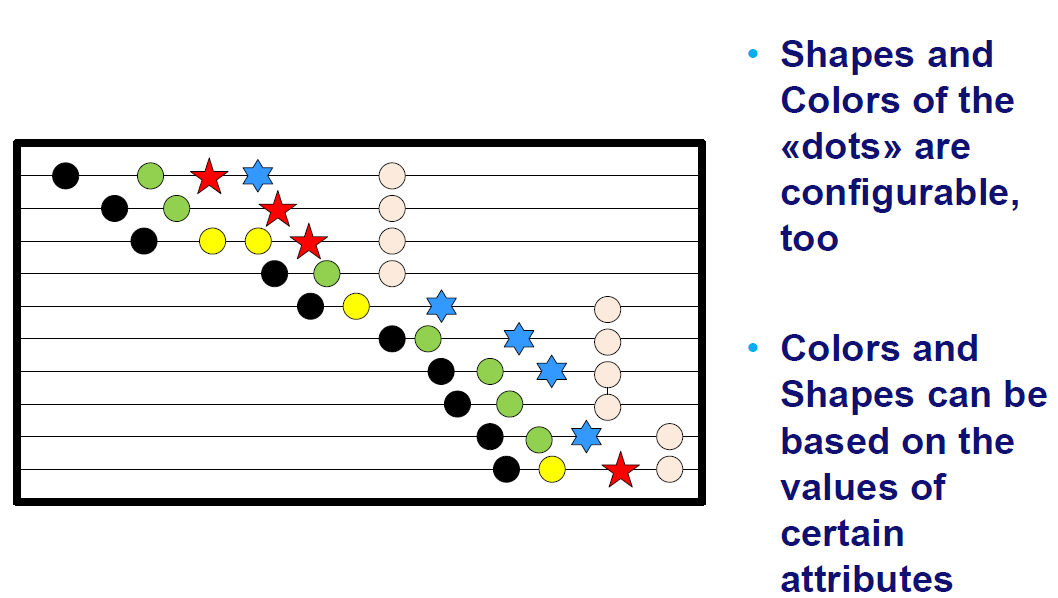
\includegraphics[width=0.7\textwidth]{capitolo 8/slide10.png}
\end{center}
For example:
\begin{itemize}
    \item Constant arrival rates,
    \item Patterns of grouped cancellations,
    \item Time-dependent changes in activity density,
    \item The amount of work each member do.
\end{itemize}
\begin{center}
    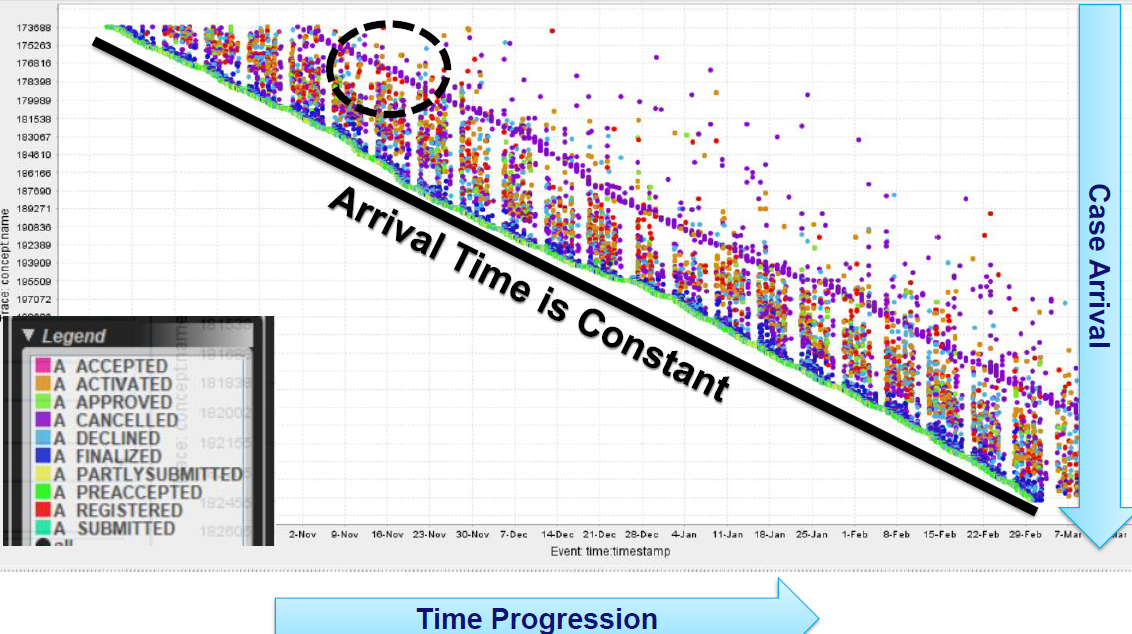
\includegraphics[width=0.7\textwidth]{capitolo 8/slide11.png}
\end{center}

\begin{center}
    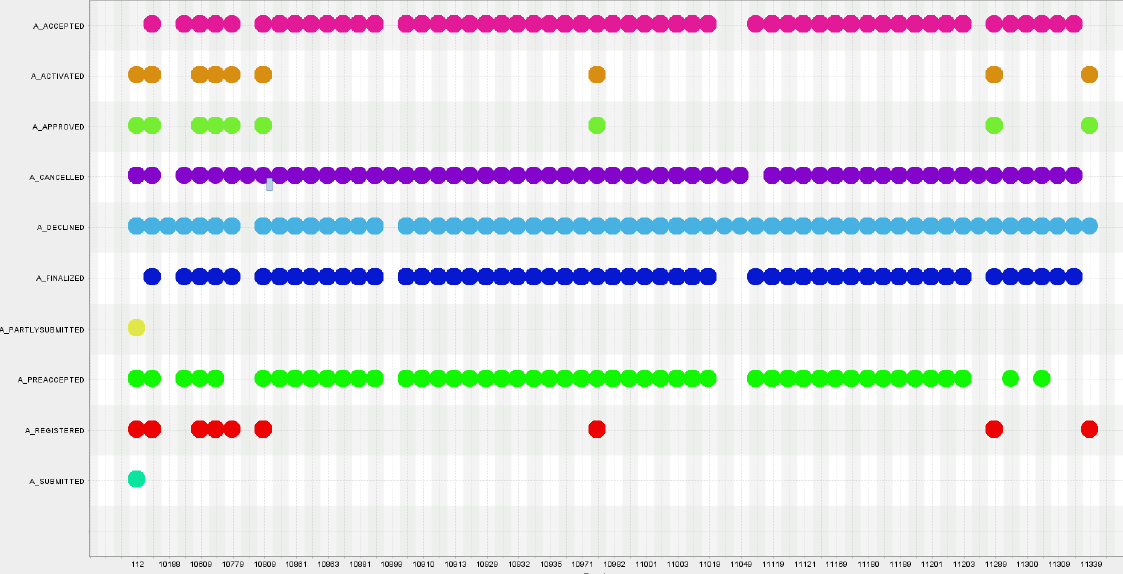
\includegraphics[width=0.7\textwidth]{capitolo 8/slide 14.png}
\end{center}

\section{Enhancing Petri Nets with Additional Perspectives}

\subsection{Resource Perspective: Organizational Mining}
The \textbf{organizational perspective} focuses on understanding people, machines, and organizational structures, such as:
\begin{itemize}
    \item Roles (e.g., manager, assistant),
    \item Departments,
    \item Work distribution among resources.
\end{itemize}

A \textbf{resource-activity matrix} records how often specific resources perform particular activities. For example:
\begin{itemize}
    \item Activity \(a\) is performed \(0.3\) times by Pete, \(0.5\) times by Mike, and \(0.2\) times by Ellen.
    \item Activities \(e\) and \(f\) are performed exclusively by Sara, often more than once per case.
\end{itemize}
\begin{center}
    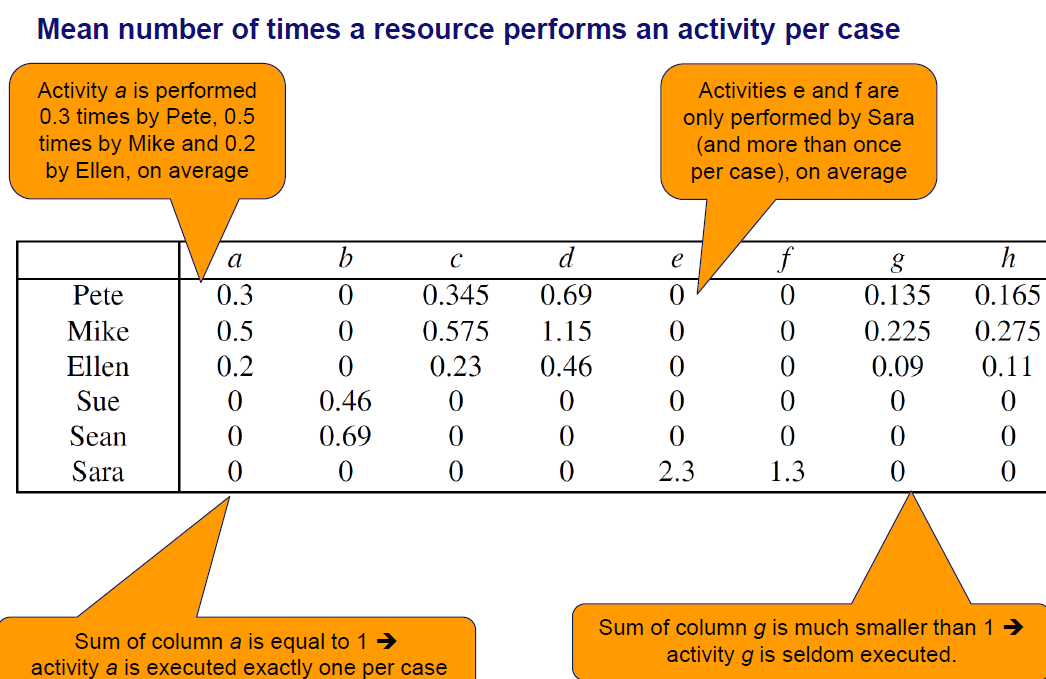
\includegraphics[width=0.7\textwidth]{capitolo 8/slide20.png}
\end{center}

Rows in the resource-activity matrix can be clustered to group resources with similar roles. Labels such as "manager," "expert," or "assistant" can be arbitrarily assigned to these clusters.

\subsection{Social Network Analysis}
Social networking techniques can visualize relationships between groups or individuals:
\begin{itemize}
    \item Nodes represent resources or roles,
    \item Arcs represent interactions (e.g., handover of work).
\end{itemize}
The size of nodes and the thickness of the arcs depend on the weight of entities and relationships, respectively.

\begin{center}
    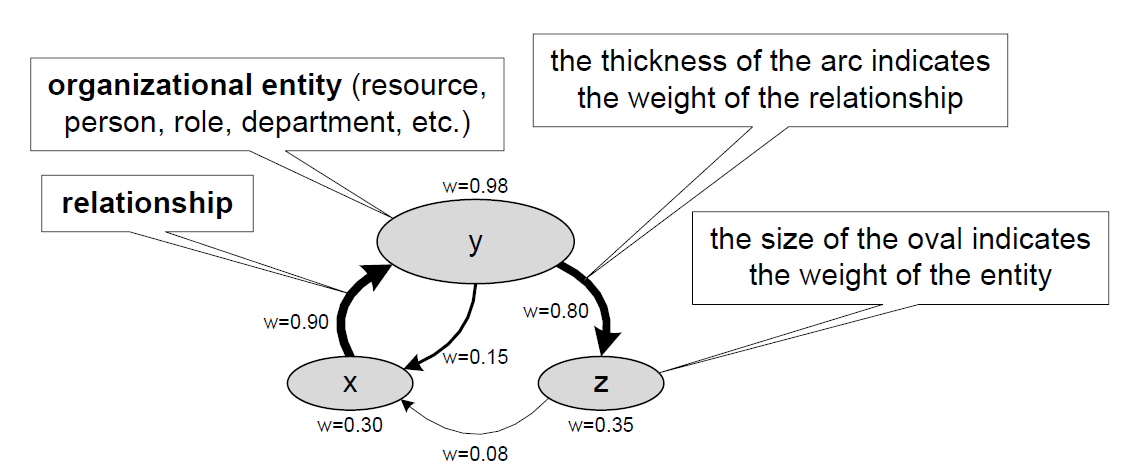
\includegraphics[width=0.7\textwidth]{capitolo 8/slide24.png}
\end{center}

\subsection{Handover of Work}
The \textbf{handover of work} represents the transfer of responsibility between resources. A direct or eventual dependency exists if:
\begin{itemize}
    \item Activity \(a_1\) is followed by \(a_2\),
    \item Or \(a_1\) indirectly influences \(a_2\) through intermediate activities.
\end{itemize}
\begin{center}
    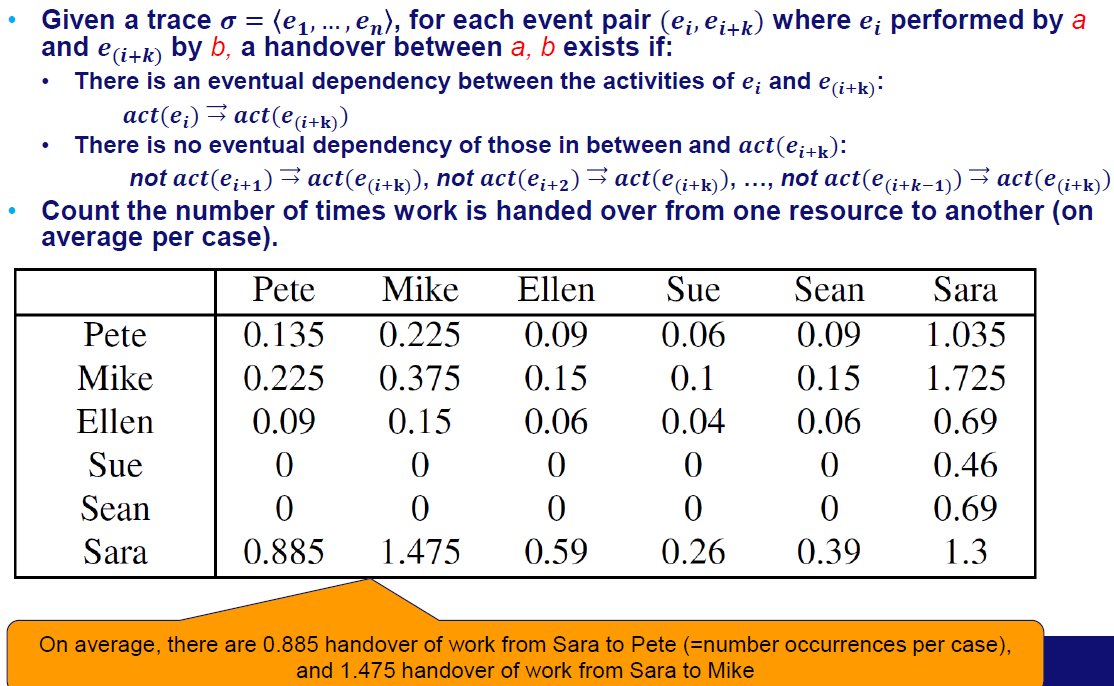
\includegraphics[width=0.7\textwidth]{capitolo 8/slide26.png}
\end{center}

\section{Data Perspective: Decision Mining}

The \textbf{data perspective} seeks to understand how choices are made between multiple paths in a process. For example:
\begin{itemize}
    \item Decision point: Choice between activities \(b\) and \(c\),
    \item Predictor variables: Resource, customer type, or monetary amount.
\end{itemize}

From the event log, patterns of decisions can be extracted. Probabilities of taking one path over another can be inferred, enabling the addition of \textbf{guards}, which specify conditions for decisions:
\[
\text{If Customer = Silver, take path \(b\); otherwise, take path \(c\)}.
\]
\begin{center}
    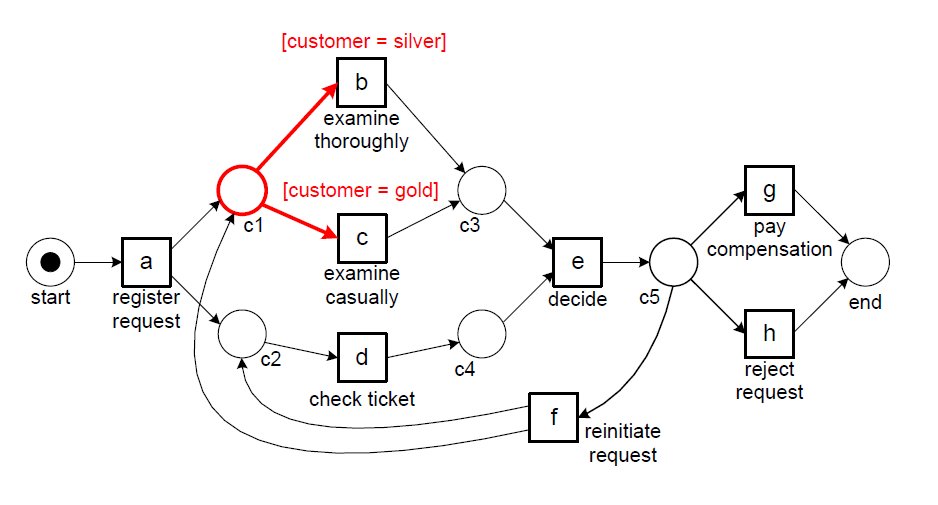
\includegraphics[width=0.7\textwidth]{capitolo 8/slide40.png}
\end{center}
We call the response variable when there is a choice, in this case between b and c. The predictor variables are attributes that are needed for the decision.

\section{Time Perspective}

The \textbf{time perspective} analyzes how long processes take:
\begin{itemize}
    \item Measure time between transitions,
    \item Identify bottlenecks where delays occur.
\end{itemize}

For example:
\begin{itemize}
    \item Long durations may indicate process blocks,
    \item Short durations suggest efficient execution.
\end{itemize}

\begin{center}
    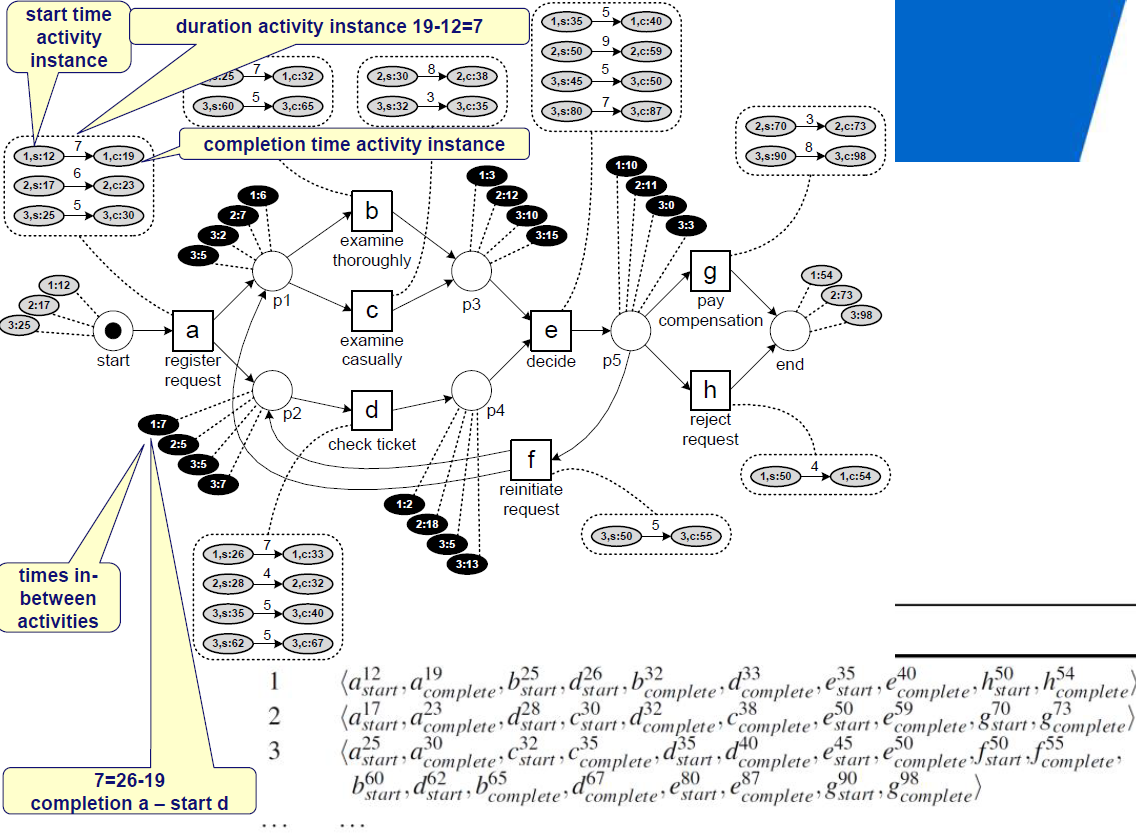
\includegraphics[width=0.7\textwidth]{capitolo 8/slide48.png}
    
\end{center}

\section{Alignments in Process Mining}

In real-world scenarios, traces may not perfectly fit the model due to:
\begin{itemize}
    \item Missing or incorrect data,
    \item Rare or exceptional cases.
\end{itemize}

\textbf{Alignments} fix traces by matching them to the "closest" path in the model, enabling:
\begin{itemize}
    \item Detection of deviations,
    \item Preservation of as much data as possible.
\end{itemize}

\section{Conclusion}

Exploring additional perspectives enriches our understanding of processes by incorporating aspects of organizational, decision, and time. This holistic approach enables more accurate and insightful process analysis, supporting better decision making and optimization.
